\documentclass[border=10pt]{standalone}

\usepackage{tikz}
\usepackage{tikzsymbols}
\usetikzlibrary{calc,patterns,shapes.geometric}

\def\centerarc[#1](#2)(#3:#4:#5){\draw[#1] ($(#2)+({#5*cos(#3)},{#5*sin(#3)})$) arc (#3:#4:#5);}

\begin{document}
	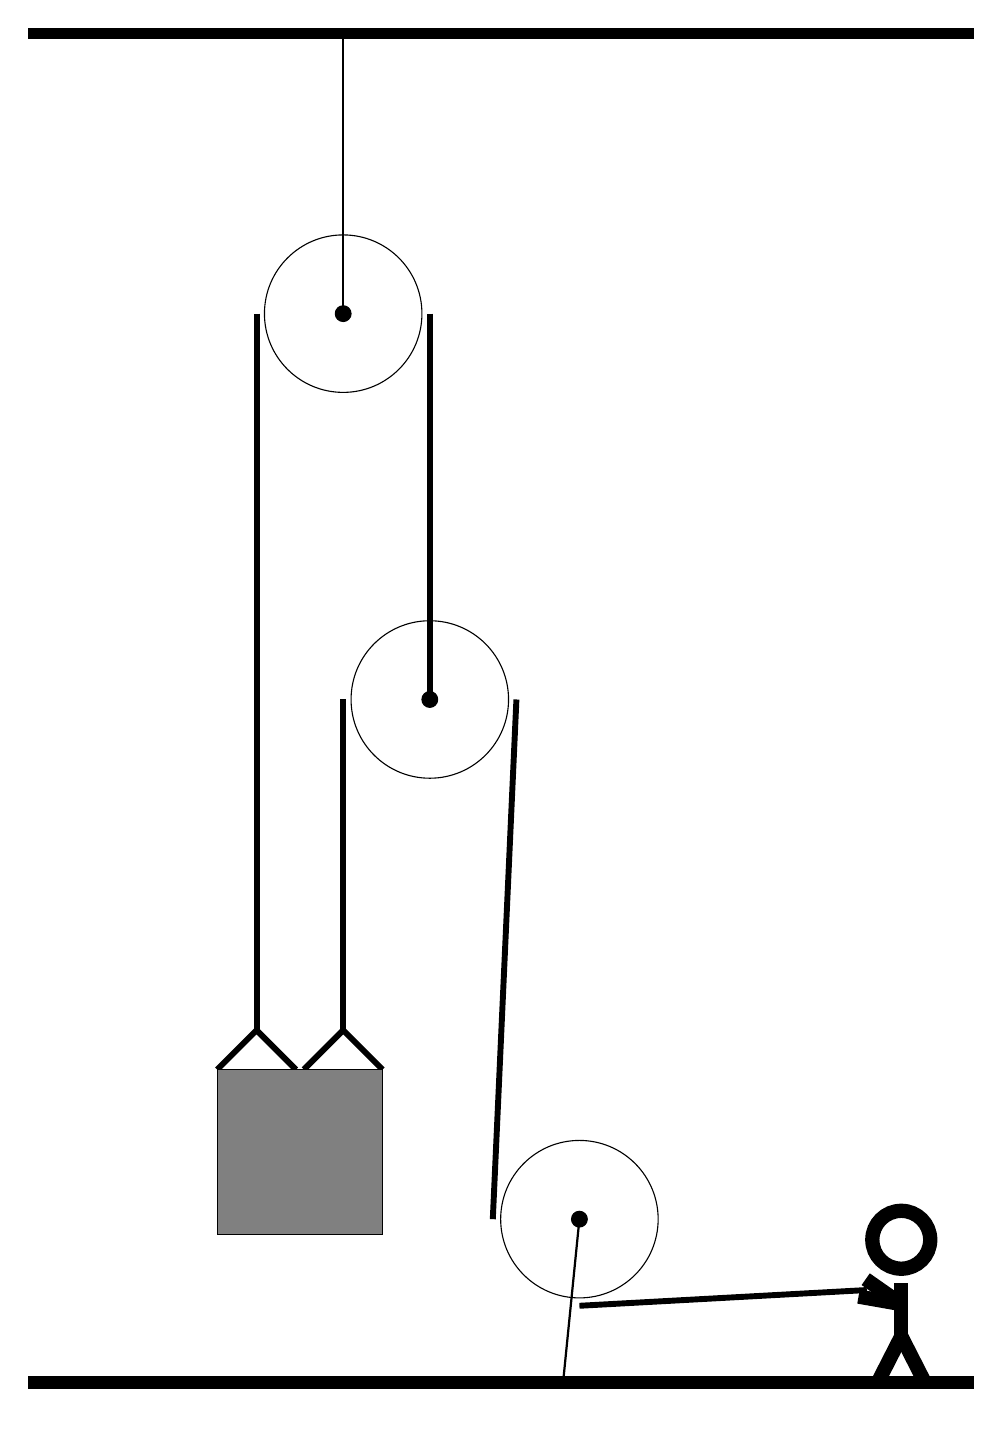
\begin{tikzpicture}
		%%%%% START %%%%%
		\draw[fill=black] (-2, 14) rectangle (10, 14.125);
		
		\draw (2, 10.5) circle (1);
		\draw[fill=black] (2, 10.5) circle (0.1);
		\draw[thick] (2, 10.5) -- (2, 14);
		
		\draw (3.1, 5.6) circle (1);
		\draw[fill=black] (3.1, 5.6) circle (0.1);
		
		\draw (5, -1) circle (1);
		\draw[fill=black] (5, -1) circle (0.1);
		\draw[thick] (5, -1) -- (4.8, -3);
		
		\draw[line width = 0.75mm]  (0.4, 0.9) -- (0.9, 1.4) -- (1.4, 0.9);
		\draw[line width = 0.75mm]  (1.5, 0.9) -- (2.0, 1.4) -- (2.5, 0.9);
		\draw[fill=black!50] (0.4, 0.9) rectangle (2.5, -1.2);
		
		\draw[line width = 0.75mm] (0.9, 10.5) -- (0.9, 1.4);
		\centerarc[line width = 0.75mm](2, 10.5)(0:180:1.1);
		\draw[line width = 0.75mm] (3.1, 10.5) -- (3.1, 5.6);
		\draw[line width = 0.75mm] (2.0, 5.6) -- (2.0, 1.4);
		\centerarc[line width = 0.75mm](3.1, 5.6)(0:180:1.1);
		\draw[line width = 0.75mm] (4.2, 5.6) -- (3.9, -1);
		\centerarc[line width = 0.75mm](5, -1)(180:270:1.1);
		\draw[line width = 0.75mm] (5, -2.1) -- (8.65, -1.9);
		
		\node at (9, -2) {\Strichmaxerl[10][-35][170]};
		
		\draw[fill=black] (-2, -3) rectangle (10, -3.15);
		%%%%% END %%%%%
	\end{tikzpicture}
\end{document}